\section{STT-RAM Cache Design Optimization} \label{sec:opt}

\begin{figure}[t]
  \centering
  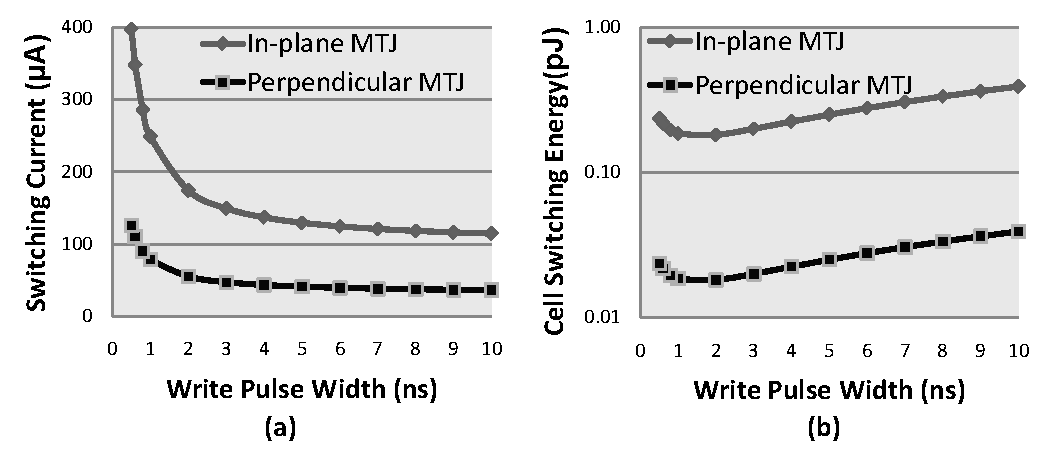
\includegraphics[width=3.5in]{fig/MTJSpec.eps}
  \caption{Representative data curves of in-plane and perpendicular MTJs: (a)Switching current; (b) Cell switching energy.}
  \label{fig:specs}
\end{figure}

\begin{figure*}[t]
  \centering
  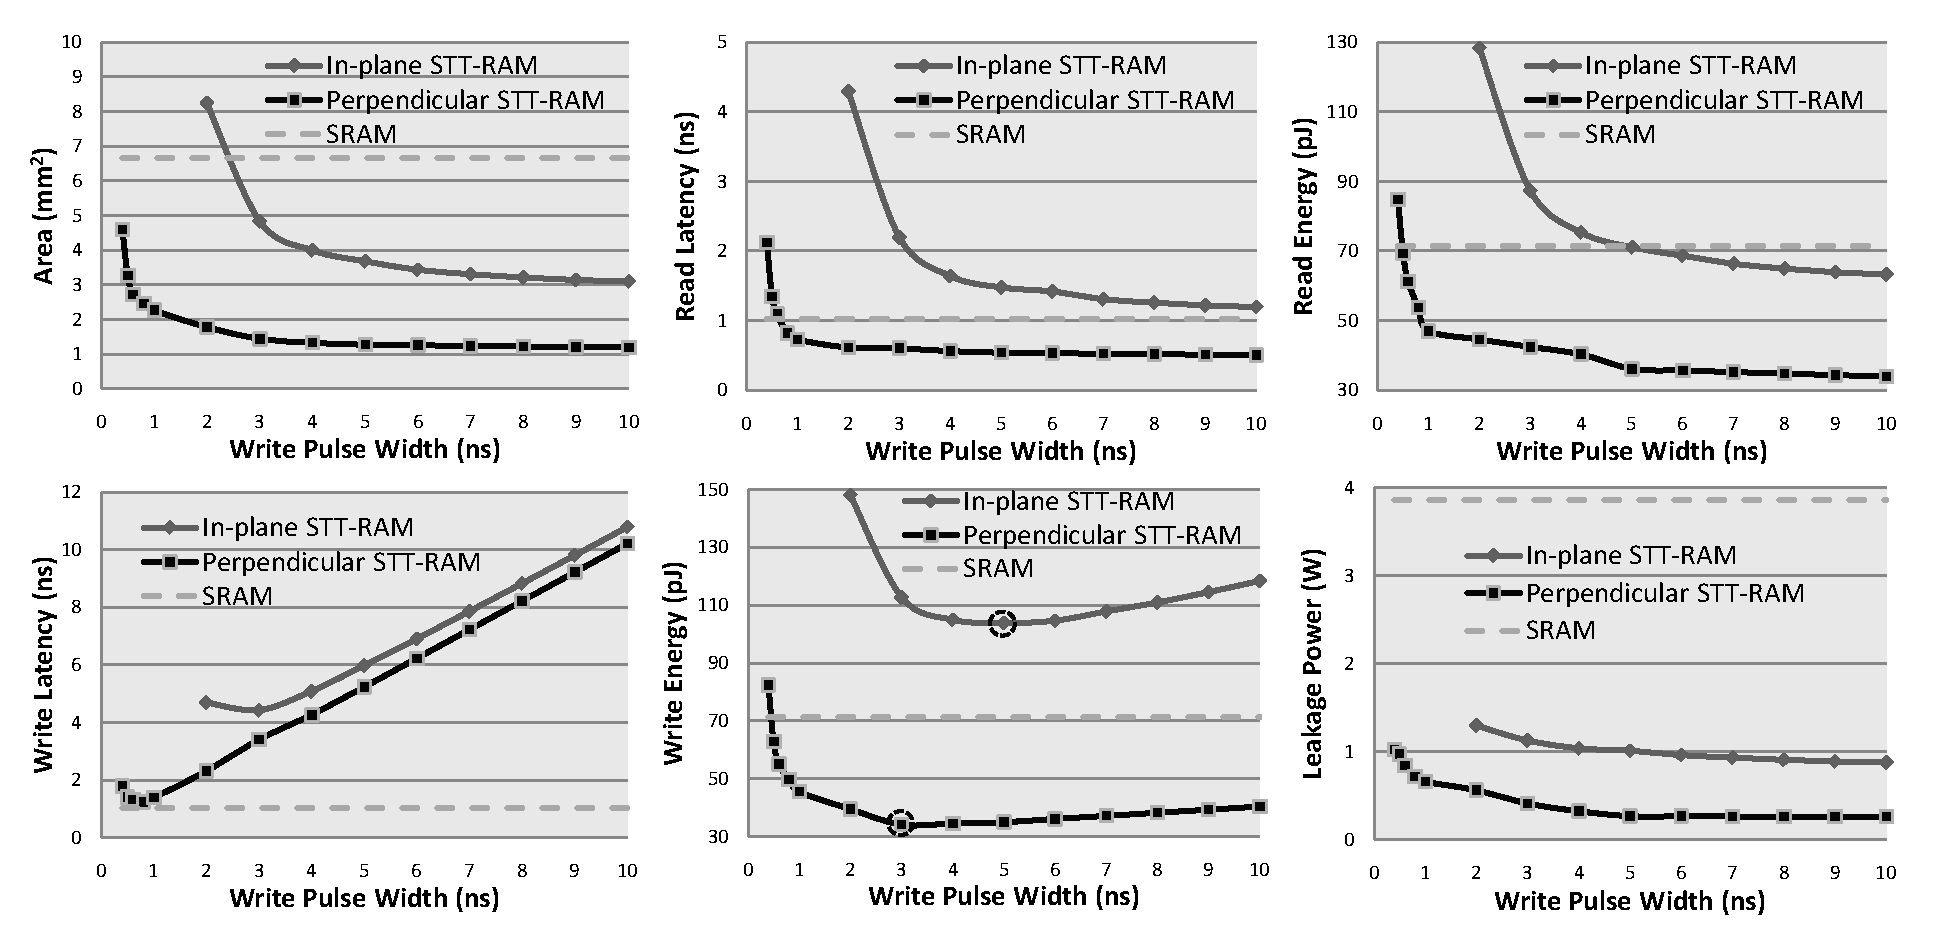
\includegraphics[width=7in]{fig/AllMetrics.eps}
  \caption{Metrics of SRAM and STT-RAM built with in-plane and perpendicular MTJs: (a)Area; (b)Read latency; (c)Read energy; (d)Write latency; (e)Write energy; (f)Leakage power.}
  \label{fig:metrics}
\end{figure*}

\begin{figure}[t]
  \centering
  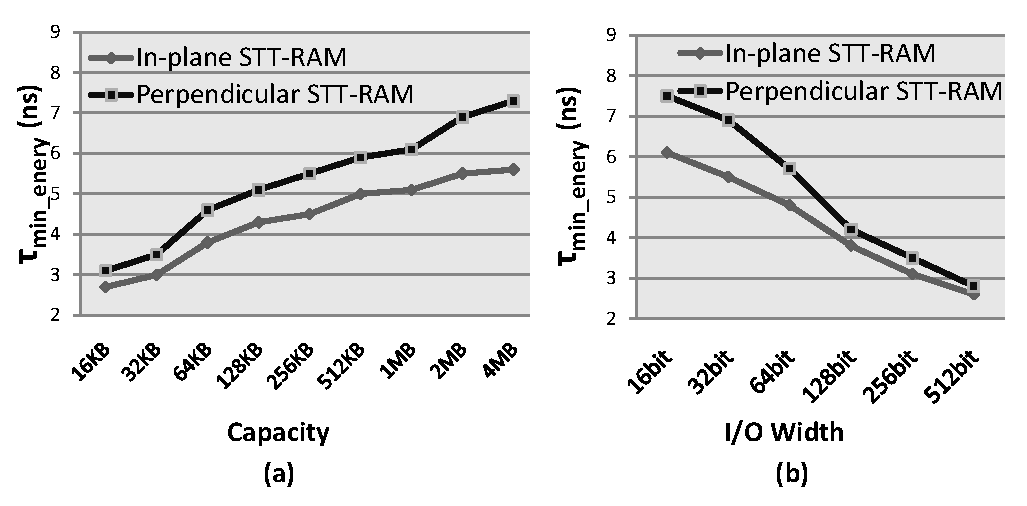
\includegraphics[width=3in]{fig/MinEnergy.eps}
  \caption{Dependence of $\tau_{min\_energy}$ on STT-RAM Macro Capacity.}
  \label{fig:minenergy}
\end{figure}

\begin{table*}[t]
%\vspace{-5pt}
\centering
\caption{Device-Architecture Co-Optimization of a 45nm 64MB STT-RAM chip}
\label{tb:bigtable}
%\vspace{-5pt}
\begin{tabular}{| l | c | c | c | c | c | c |}
\hline\hline
& Area opt. & Read latency opt. & Write latency opt. & Read energy opt. & Write energy opt. & Leakage opt. \\
\hline
Area ($mm^2$) & \textbf{3.06} & 10.7 & 16.4 & 5.66 & 6.22 & 3.63 \\
\hline
Read latency ($ns$) & 21.8 & \textbf{3.70} & 4.92 & 9.12 & 9.57 &	9.91 \\
\hline
Write latency ($ns$) & 18.6	& 13.9	& \textbf{4.0}1	& 15.9	& 11.3	& 18.1 \\
\hline
Read energy ($nJ$) & 0.276	& 0.225	& 0.316	& \textbf{0.105}	& 0.139	& 0.279 \\
\hline
Write energy ($nJ$) & 0.293	& 0.322	& 0.309	& 0.193	& \textbf{0.131}	& 0.281\\
\hline
Leakage ($W$) & 1.01	& 3.53	& 4.98	& 1.85	& 1.92	& \textbf{0.78}\\
\hline\hline
Write pulse width ($ns$) & 10 & 10 & 2 & 10 & 5 & 10 \\
\hline
Inter-array routing & Non-H-tree & H-tree & H-tree & H-tree & H-tree & Non-H-tree \\
\hline
Sense amp placement & External & Internal & Internal & Internal & Internal & External \\
\hline
Sense amp type & Current-in voltage & Current & Current & Voltage-divider & Voltage-divider & Voltage-divider \\
\hline
Interconnect wire & Normal & Repeated & Repeated & Low-swing & Low-swing & Normal \\
\hline
Output buffer type & Area opt. & Latency opt. & Latency opt. & Area opt. & Area opt. & Area opt. \\
\hline\hline
\end{tabular}
%\vspace{-10pt}
\end{table*}